\documentclass[a4paper]{llncs}
\usepackage[T1]{fontenc}
\usepackage[utf8]{inputenc}
\usepackage{authblk}
\usepackage{graphicx, epstopdf, color, setspace, algorithm, amsfonts, amsmath, mathtools, nicefrac}
\usepackage[algo2e, noend, noline, linesnumbered]{algorithm2e}
\SetKwIF{If}{ElseIf}{Else}{if}{then}{else if}{else}{endif}
\newcommand{\func}[1]{{\sc #1}}
\newcommand{\tuple}[1]{\ensuremath{\left \langle #1 \right \rangle }}
\DontPrintSemicolon
\DeclarePairedDelimiter{\ceil}{\lceil}{\rceil}
\DeclarePairedDelimiter{\floor}{\lfloor}{\rfloor}
\newcommand{\eg}{{\it e.g.,}~}
\newcommand{\ie}{{\it i.e.,}~}
\newcommand{\bE}{\mathbb{E}}
\newcommand{\cf}{{cf.}~}
\newcommand{\TODO}[1]{\textbf{\color{red}#1}}
\graphicspath{{img/}}
\pagestyle{headings}
\title{Minimizing~Simple~and~Cumulative~Regret in~Monte-Carlo~Tree~Search}

\author{Tom~Pepels\inst{1} \and Tristan~Cazenave\inst{2} \and
Mark~H.M.~Winands\inst{1} \and Marc~Lanctot\inst{1}}

\institute{Department of Knowledge Engineering,  Maastricht University\\ \email{\{tom.pepels,m.winands,marc.lanctot\}@maastrichtuniversity.nl} \and LAMSADE - Université Paris-Dauphine \\ \email{cazenave@lamsade.dauphine.fr}}


\begin{document}

\maketitle

\begin{abstract} Regret minimization is key to both the Multi-Armed Bandit problem and Monte-Calo Tree Search (MCTS). Recently, simple regret, the regret of not having recommended the best action, has been proposed as an alternative to cumulative regret, regret accumulated over time. Each type of regret is appropriate in different contexts. In this paper, a new MCTS variant named Hybrid MCTS (H-MCTS) is proposed, which minimizes both types of regret. H-MCTS uses UCT to minimize cumulative regret, and a recursive version of Sequential Halving, named SHOT to minimize simple regret near the root. Moreover, we show the performance of H-MCTS in $X$ different games: game1, game2, ...

\end{abstract}

\section{Introduction}
\label{sec:intro}

The driving force behind MCTS is the notion of regret minimization. Algorithms used in MAB research have been developed to minimize \emph{cumulative regret}. Cumulative regret is the expected regret of not having sampled the optimal decision in hindsight. This type of regret is accumulated during execution of the algorithm, each time a non-optimal arm is sampled the cumulative regret increases. UCB1~\cite{auer2002using} is a selection policy for the MAB problem, which minimizes cumulative at a fast rate, converging to the empirically best arm fast. Once the best arm is found by exploring the available options, it exploits it by repeatedly pulling that arm, minimizing overall cumulative regret. This policy was adapted to be used in MCTS in the form of UCT~\cite{kocsis2006bandit}.

The Multi-Armed Bandit (MAB) problem is defined as a stochastic decision making problem~\cite{auer2002using}. An agent is faced with several options, each with their own reward distribution. Based on sampling the search space an agent is to select the option with the best reward distribution. Generally the problem is described as choosing between the most rewarding arm of a multi-armed slot machine found in casino's. The agent can explore by pulling an arm and observing the resulting reward. The reward is drawn from either a fixed or changing probability distribution. Each pull and the returned reward constitutes a sample.

Recently, \emph{simple regret} has been proposed as a new criterion for assessing the performance of both MAB~\cite{audibert2010best,Bubeck11Pure} and MCTS~\cite{tolpin2012mcts,Feldman12BRUE,Cazenave14SHOT} algorithms. Simple regret is defined as the expected error between an algorithm's recommendation, and the optimal decision. A naturally fitting quantity to optimize in the MCTS setting, since all simulations executed by MCTS are for the mere purpose of learning good moves. However, the final move chosen after all simulations are performed, \ie the \emph{recommendation}, is the one that has real consequence. However, since the introduction of Monte-Carlo Tree Search (MCTS)~\cite{kocsis2006bandit} and its subsequent adoption by games researchers~(\cf~\cite{browne2012survey}) UCT~\cite{kocsis2006bandit}, or some variant thereof, has become the ``default'' selection policy. 

\vspace{2mm}
In this paper, we present a new, hybrid MCTS technique that utilizes both UCT, and the recently introduced Sequential Halving~\cite{Karnin13SH}. As such, the new technique, named Hybrid MCTS (H-MCTS) uses both simple, and cumulative regret minimizing policies to their best effect. We empirically show our results in \TODO{$X$ games: bla, bla, and bla.}

The paper is structured as follows, first MCTS and UCT are introduced in Section \ref{sec:mcts}, next in Section~\ref{sec:reg_min} a recently introduced, simple regret minimizing technique for the MAB problem, Sequential Halving~\cite{Karnin13SH}, is discussed. Sequential Halving is used recursively in SHOT~\cite{Cazenave14SHOT} which is described in detail in Section~\ref{sec:shot}. Together, SHOT and UCT form the basis for the new, hybrid MCTS technique discussed in Section~\ref{sec:h-mcts}. This is followed by the experiments, in Section~\ref{sec:exp_res} and finally by the conclusion and an outline of future research, in Section~\ref{sec:concl}.

\section{Monte-Carlo Tree Search}
\label{sec:mcts}

Monte-Carlo Tree Search (MCTS) is a best-first search method based on random sampling by Monte-Carlo simulations of the state space of a domain~\cite{coulom2007efficient,kocsis2006bandit}. In gameplay, this means that decisions are made based on the results of randomly simulated play-outs. MCTS has been successfully applied to various turn-based games such as Go~\cite{lee2010current}, Lines of Action~\cite{Winands2010b}, and Hex~\cite{arneson2010monte}. Moreover, MCTS has been used for agents playing real-time games such as the Physical Travelling Salesman~\cite{powleytsp}, real-time strategy games~\cite{balla2009uct}, and Ms~Pac-Man~\cite{realtime2014}, but also in real-life domains such as optimization, scheduling, and security~\cite{browne2012survey}.

In MCTS, a tree is built incrementally over time, which maintains statistics at each node corresponding the rewards collected at those nodes and number of times they have been visited. The root of this tree corresponds to the current position. As such, MCTS can be considered a recursive multi-armed bandit. The basic version of MCTS consists of four steps, which are performed iteratively until a computational threshold is reached, \ie a set number of simulations, an upper limit on memory usage, or a time constraint. 

Each MCTS simulation consist of two main steps, 1) the \emph{selection} step, where moves are selected and played inside the tree according to the selection policy until a leaf is \emph{expanded}, and 2) the \emph{play-out}, in which moves are played according to a simulation policy, outside the tree. At the end of each play-out a terminal state is reached and the result is \emph{backpropagated} along the tree from the expanded leaf to the root.

\subsection{UCT}
\label{subsec:uct}
During the selection step, a policy is required to explore the tree to decide on promising options. For this reason, the widely used Upper Confidence Bound applied to Trees (UCT)~\cite{kocsis2006bandit} was derived from the UCB1~\cite{auer2002using} policy. In UCT, each node is treated as a bandit problem whose arms are the moves that lead to different child nodes. UCT balances the exploitation of rewarding nodes whilst allowing exploration of lesser visited nodes. Consider a node $p$ with children $I(p)$, then the policy determining which child $i$ to select is defined as:

\begin{equation}
\label{eq:uct}
i^* = argmax_{i \in I(p)}\left\{ v_i + C \sqrt{ \frac{\ln{n_p}}{n_i}}\right\},
\end{equation}
where $v_i$ is the score of the child $i$ based on the average result of simulations that visited it, $n_p$ and $n_i$ are the visit counts of the current node and its child, respectively. $C$ is the exploration constant to tune. UCT is applied when the visit count of a child node is above a threshold $T$. When a node's visit count is below this threshold, a child is selected at random.

Note that, UCB1 and, consequentially UCT incorporate both exploitation, and exploration. After a number of trials, a node that is identified as the empirical best is selected more often. In tree-search this has three consequences:
\begin{enumerate} 

\item Whenever a promising move is found, less time is spent on suboptimal moves. Since MCTS is generally time bounded it is important to spend as much time as possible exploring the best moves. Because, by the \emph{MinMax} principle in two-player games, at each ply we expect a player to maximize the minimum gain.

\item The valuation of any node in the tree is dependent on the values back-propagated. Given that UCT spends the least possible time on suboptimal moves, any values back-propagated are based on increasingly better approximations of simulations performed deeper in the tree. In fact, given infinite time, UCT converges to selecting only moves with the highest average values.

\item The current value of the node can be falsified by searching deeper. In MCTS, each simulation increases the depth of the search, and as such may reveal moves as becoming worse over time due to an unpredicted turn of events. If an expected good move is not reselected often, such ``traps''~\cite{Ramanujan2010a} are not revealed.

\end{enumerate}

\section{Regret}
\label{sec:regret}
In this section we will discuss regret in both the MAB, and MCTS context. The differences between cumulative and simple regret are discussed in Subsection \ref{subsec:cumsimregret}. Next we discuss regret in the context of MCTS, in Subsection \ref{subsec:reg_mcts}.

\subsection{Cumulative and Simple Regret}
\label{subsec:cumsimregret}

Suppose a trial is set-up such that a forecaster (a player, or agent) has $i \in [[K]] = \{ 1, 2, \cdots , K \}$ actions which can be repeatedly sampled over $n \in \{ 1, 2, \cdots, T \}$ trials. Each arm has an expected reward $\mu_i$, and there exists a single optimal arm with expected reward $\mu^*$.Suppose further that the forecaster employs a selection policy $I(n)$ which outputs some $a$ to be sampled at time $n$, and a recommendation policy $J(n)$ which selects the best arm at $T$.

\emph{Cumulative regret} is defined as the regret of having not sampled the best single action in hindsight, 
\begin{equation}
R_n = \sum_{t = 1}^{n}{\mu^* - \mu_{I(t)}}.
\end{equation}
In other words, the regret is accumulated over time, for each sample the forecaster takes.

Now suppose that we change the experimental set-up, such that the actions chosen on trials $1, 2, \ldots, T-1$ are taken under some realistic ``simulated environment'' that represents the true on-line decision problem but without committing to the actions. The only \emph{real} decision is made at step $T$ after having played $T-1$ simulations. In contrast, \emph{simple regret}~\cite{Bubeck11Pure} quantifies only the regret for the recommendation policy $J$ at time $T$,

\begin{equation}
r_n = \mu^* - \mu_{J(n)},
\end{equation}
\ie the regret of not having recommended the best action.

In their analysis of the links between simple and cumulative regret~\cite{Bubeck11Pure} found that upper bounds on $R_n$ lead to lower bounds on $r_n$, and that the smaller the upper bound on $R_n$, the higher the lower the lower bound on $r_n$, regardless of the recommendation policy, \ie the smaller the cumulative regret, the larger the simple regret. As such, no policy can give an optimal guarantee on both simple and cumulative regret at the same time. In the case of an MAB, the strategy used depends on the context of the problem.

\subsection{Regret in MCTS}
\label{subsec:reg_mcts}

Based on the analysis in the Subsection~\ref{subsec:uct}, the minimization of cumulative regret is naturally suitable to tree search, and the UCB1 selection policy can be used nearly unaltered in this setting as UCT. However, there exist two contexts for the multi-armed bandit problem, also to be considered in MCTS. These are:

\begin{enumerate}

\item Each trial results in a direct reward for the agent. As such we want to minimize the number of suboptimal arms pulled in order to achieve an as high as possible reward. This relates, for example, to slot machines in a casino. Every choice made at each point in the algorithm has a direct effect on the agent's reward. In this case, the reward of the agent is inversely proportional to its \textbf{cumulative regret}.

\item The agent can perform a number of trials, without consequence, in a simulated environment. The agent is allowed $T$ trials in this fashion, after which it must make a recommendation. Based on its recommendation, the agent is rewarded. In this case, the performance of the agent is measured by the \textbf{simple regret} of its recommendation. A low simple regret implies that the recommendation is close to the actual best option.

\end{enumerate}

In most MCTS literature, UCT is used as selection policy~(\cf~\cite{browne2012survey}), suggesting that the first context applies. However, the second context is a more natural fit when MCTS is used to play games. Because the behaviour of the agent in the domain is based solely on its recommendations. 
However, simulations in MCTS do have an immediate impact on its performance. Since MCTS must make a recommendation in a finite amount of time, spending more time on sub-optimal moves decreases time available to explore those expected to have high utility. This was also shown in~\cite{tolpin2012mcts} where the authors use a measure based on the Value of Information (VOI) to determine whether to exploit an expected good move.

\section{Regret Minimization}
\label{sec:reg_min}

Non-exploiting selection policies have been proposed to decrease simple regret at high rates. Given that UCB1~\cite{auer2002using} has an optimal rate of cumulative regret convergence, and the conflicting limits on the bounds on the regret types shown in~\cite{Bubeck11Pure}, policies that have a higher rate of exploration than UCB1 will have better bounds on simple regret.

\subsection{Sequential Halving}
\label{subsec:seq_halving}

Consider a uniform selection policy that samples each arm of an MAB $|K|/T$ times. Assuming that there are $h$ best arms, $(|K|-h)/T$ simulations are spent on inferior arms, and $h/T$ on the best one(s). In games for instance, there are often only one or two good moves to be identified, and therefore, when using uniform selection, most time is wasted on pulling sub-optimal arms. Therefore, a more efficient policy is required to ensure that inferior arms are not selected as often as arms with a high utility over time. Successive Rejects~\cite{audibert2010best} was the first algorithm to show a high rate of decrease in simple regret. It works by dividing the total computational budget into distinct rounds. After each round, a single arm is removed from selection, and the algorithm is continued on the reduced subset. Sequential Halving~\cite{Karnin13SH}, discussed in Subsection~\ref{subsec:seq_halving}, was introduced later as an alternative to Successive Rejects, offering better performance in large-scale MAB problems.

A recently introduced algorithm for MAB, Sequential Halving~\cite{Karnin13SH} (SH) minimizes simple regret more efficiently and ensures suboptimal arms are sampled minimally. SH divides search time into distinct rounds, and during each round arms are sampled uniformly. After each such round, half the remaining arms are removed each time until a single one remains. The rounds are equally distributed such that each round has the same number of trials (budget), but with a lower number of available arms. Sequential Halving is detailed in Algorithm~\ref{alg:seqhalv}.

\IncMargin{1em}
\RestyleAlgo{boxruled}
\begin{algorithm2e}[ht]
	\KwIn{total budget $T$, arms $K$}
	\KwOut{recommendation $J_T\in K$}
	\vspace{0.1cm}
	$S_0 \gets \{1,\dots,K\}$,
	$B \gets \ceil{\log_2{|S|}} - 1$														\;
	\BlankLine
	\For{k=0 \emph{\KwTo} $B$}{
		sample each arm $i \in S_k$, 										
		$n_k = \displaystyle\floor[\bigg]{\frac{T}{|S_k|\ceil{\log_2{|S|}}}}$
		times 																				\;
		\vspace{0.1cm}
		$S_{k+1} \gets$ the $\ceil{|S_k|/2}$ arms from $S_k$ with the highest empirical average		\;																		\;
	}
	\KwRet{the single element of $S_k$}
  \caption[Sequential Halving]{Sequential Halving~\protect\cite{Karnin13SH}. \label{alg:seqhalv}}
\end{algorithm2e}
\DecMargin{1em}

In the next section a recently introduced MCTS technique is detailed which uses SH recursively. This algorithm is the basis for H-MCTS discussed in Section~\ref{sec:h-mcts}.

\section{Sequential Halving Applied to Trees}
\label{sec:shot}

\section{A Hybrid MCTS}
\label{sec:h-mcts}

Recall that the MAB context, in which simple regret minimization is appropriate, only the final recommendation made by an algorithm has effect on the agent's reward. In gameplay this holds for the nodes of the search tree at the first ply. Only after running simulations is a recommendation made which affects the state of the game being played. Nodes deeper in the tree have an implicit effect on this decision. Because the shape of an MCTS tree is directly related to the potential reward of internal nodes, promising nodes are selected more often to grow the tree in their direction. This both enforces the confidence of the reward of promising nodes, but also ensures that their reward can be falsified based on results deeper in the tree.

\begin{figure}[ht]
	\centering
	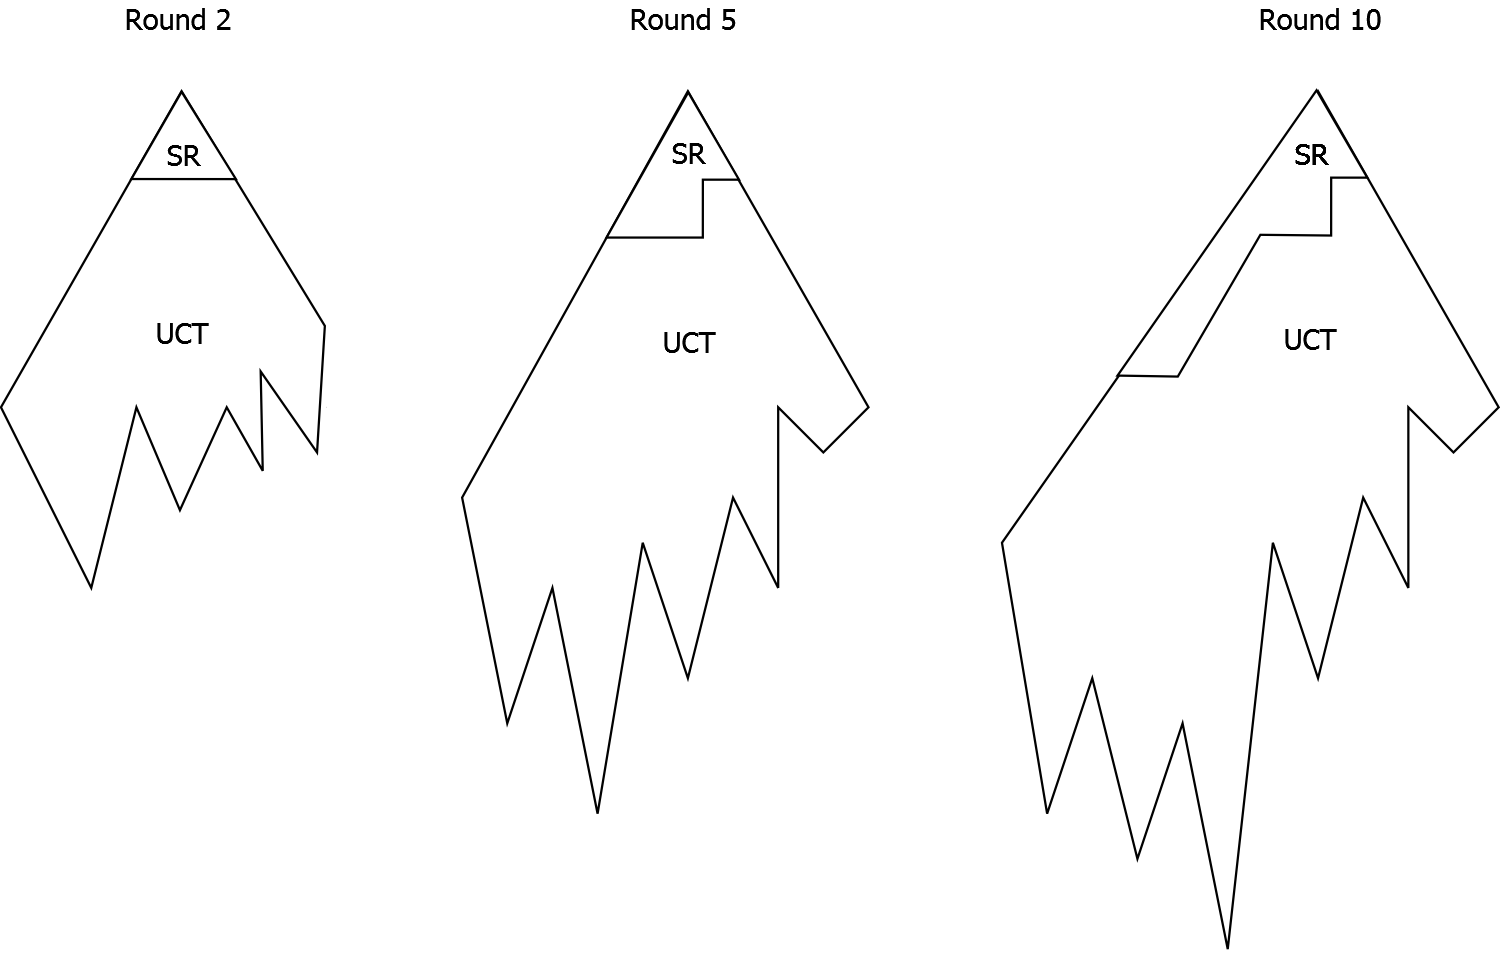
\includegraphics[width=.8\textwidth]{img/H-MCTS.png}
	\caption{Example progression of H-MCTS. In the top part of the tree (SR), simple regret is minimized, in the lower part UCT minimizes cumulative regret. The rounds represent the Sequential Halving round at the root.}
	\label{fig:h-mcts_trees}
\end{figure}

Treating a game tree as a recursive multi-armed bandit thus reveals different objectives for the distinct plies of the tree. At the root, simple regret should be as low as possible, since the recommendation of the algorithm is based on the first ply of the tree. On deeper plies, we want to both sample efficiently, avoiding time wasted on bad options, and back-propagate correct values from leafs to their ancestors. Where the former can be achieved by using selection policies such as Successive Rejects or Sequential Halving, the latter, as discussed in Section~\ref{sec:mcts} is inherently performed by UCT. Intuitively, this leads to the belief that we should only minimize simple regret at the root, and use UCT throughout of the tree. However, considering that at any ply, based on the MinMax principle, we want to find the \emph{best reply} to the action of the parent. It may also be beneficial to ensure a low simple regret on that particular move. Because this intrinsically leads to an improved evaluation of the parent.

Using a selection policy based on both SHOT and UCT, Hybrid MCTS (H-MCTS) combines simple and cumulative regret minimization in a tunable algorithm. Based on the results in~\cite{Bubeck11Pure}, which show that given a low sampling budget, UCB empirically realizes lower simple regret. The proposed technique switches from UCT to Sequential Halving whenever the computational budget is above the budget limit $B$. Consequently, the search tree is composed of a \emph{simple regret tree} at the root, and \emph{UCT trees} rooted at the leafs of the simple regret tree. As shown in Figure~\ref{fig:h-mcts_trees}, initially the simple regret tree is shallow because the computational budget per node is small. Later, when the budget per node increases due to nodes being removed from selection as per Sequential Halving, the simple regret tree grows deeper. Note that, since the root's children are sorted in descending order, the right part of the simple regret and UCT tree is always the deepest, since it its root is selected the most.
\IncMargin{1em}
\begin{algorithm2e}[t]
\setstretch{1.1}
	\KwIn{node $p$, allocated budget $budget$}
	\KwOut{$t_s$: number of play-outs, $p1$ and $p2$ wins, budget spent}
	\func{h-mcts}(node $p$, $budget$):													\;
	\Indp
	\lIf{isLeaf($p$)}{$S\gets$ \func{expand}($p$)}					
	$t_s \gets \tuple{0,0,0,0}$															\;		
	\If{isTerminal($p$)}{																	\label{h-mcts:terminal}
		\func{update} $t_s$, with $budget$ wins and $budget$ visits, 
		\KwRet{$t_s$}																	\;
	}
	$s \gets |S|$																		\;
	$b \gets \displaystyle\max{\left(1, \floor[\bigg]{\frac{p.budgetSpent + budget}{s\times\ceil{log_2{s}}}}\right)}$ \; \label{h-mcts:budgetlimit}
	\If{$p$ is not root \textbf{and} $b < B $}{
		\For{i=0 \emph{\KwTo} budget}{
			$\tuple{v, w_1, w_2, b_{u, p}}_i \gets$ \func{uct}($p$)						\;
			\func{update} $t_s$ with $\tuple{v, w_1,w_2, b_{u, p}}_i$					\;
		}
		\KwRet{$t_s$}
	}
	$b_u, k \gets 0$, $S_0 \gets S$																		\;
	\Repeat{s $=$ 1 \textbf{or} $b_u >= budget$} {										\label{h-mcts:shot}
		\For{i=0 \emph{\KwTo} s}{
			$n_i \gets$ node $n$ at rank $i$ of $S_k$								\;
			$b_i \gets b - n_i.visits$												\;
			\If{$b_i > 0$} {
				\If{$p$ is root \textbf{and} $i = 0$ \textbf{and} $s = 2$} {
					$b_i \gets \max{(b_i, budget - b_u - (b - n_1.visits))}$					\;
				}
				$b_i \gets \min{(b_i, budget - b_u)}$									\;
				$\tuple{v, w_1, w_2, b_{u, n_i}}_i \gets$ \func{h-mcts}($p$, $b_i$)		\;
				\func{update} $p, b_u,$ and $t_s$ with $\tuple{v, w_1, w_2, b_{u, n_i}}_i$		\;
			}
			break if $b_u \geq budget$												\;
		}
		$s \gets \ceil{\nicefrac{s}{2}}$, $k \gets k + 1$							\;
		$S_{k} \gets$ the $s$ arms from $S_{k-1}$ with the empirically best average	\;	\label{h-mcts:sort}
		$b \gets b + \displaystyle\max{\left(1, \floor[\bigg]{\frac{p.budgetSpent + budget}{s\times\ceil{log_2{s}}}}\right)}$ \;	
	}
	\func{update} $p.budgetSpent$ with $b_u$										\;
	\Indm
	\KwRet{$t_s$}
  \caption{Hybrid Monte-Carlo Tree Search (H-MCTS). \label{alg:h-mcts}}
\end{algorithm2e}
\DecMargin{1em}

H-MCTS is outlined in Algorithm~\ref{alg:h-mcts}. Similar to UCT and SHOT on line~\ref{h-mcts:terminal} terminal conditions are handled. Followed by the main feature of the algorithm on line~\ref{h-mcts:budgetlimit} where the initial simulation budget $b$ for each child of the current node is computed. Based on $b$, a decision is made whether to progress into the UCT tree if $b<B$ or, if $b >= B$ to continue with SHOT. Note that, the $b<B$ check is overridden at the root, since only one cycle is initiated there, and because at the root simple regret minimization is always favoured over cumulative regret minimization. From line~\ref{h-mcts:shot} the algorithm is similar to the Sequential Halving potion of SHOT. As in SHOT, because multiple play-outs are back-propagated in a single descent from root to leaf, the algorithm returns a tuple $t_s$, which contains: 1) the budget used $b_u$, 2) the number of wins per player $w_1$ and $w_2$, and 3) the number of visits $v$. UCT also maintains this tuple such that is can return the same $t_s$ to the simple regret tree. However, in the case of UCT all values in $t_s$ are at most 1. For the UCT tree, any implementation can be used, as long as it is adapted to return $t_s$ and update the $budgetSpent$ value alongside the usual node's visit count. Because any UCT node in the tree can be ``converted'' to a simple regret node at any time, when $b>B$ on line~\ref{h-mcts:budgetlimit}.

H-MCTS shares its disadvantage of not being able to return a recommendation at any-time with SHOT. It must know its exact computational budget beforehand. However, it does makes use of the fact that UCT is any-time. Suppose a node was selected and expanded by H-MCTS, then at each time in the simple regret tree, nodes will have an appropriate value based on the results back-propagated by UCT. Thus, when SHOT finishes a round by sorting the nodes by their accumulated values on line~\ref{h-mcts:sort}, UCT's any-time property ensures nodes have a representative value.

To a lesser extent, H-MCTS also shares the speed benefit of SHOT. However, because a large part of the search tree is composed of the UCT tree, based on the budget limit $B$ H-MCTS will still spend more time in the tree than SHOT overall.

\section{Experiments and Results}
\label{sec:exp_res}

\section{Conclusion}
\label{sec:concl}

\subsection*{Acknowledgements} 
This work is partially funded by The Netherlands Scientific Research (NWO) in the framework of the project Go4Nature, grant number 612.000.938.

\bibliographystyle{splncs03}
\bibliography{h-mcts}
\end{document}